\chapter{Introduction}\label{ch-introduction}
\thispagestyle{headings}
\markboth{Chapter \ref{ch-introduction}: Introduction}{Chapter \ref{ch-introduction}: Introduction}

QUESO is a parallel object-oriented statistical library dedicated to the research of statistically robust, scalable, load balanced, and fault-tolerant mathematical algorithms for the quantification of uncertainty (UQ) of mathematical models and their predictions. 
% It has been developed to implement advanced algorithms for Bayesian
% inference, including are many variants of MCMC and the multi-level algorithm.  It is able to handle uni- and multi-processor Linux
% environments and to provide a wide range of diagnostics.


The purpose of this chapter is to introduce relevant terminology, mathematical and statistical concepts, statistical algorithms, together with an overall description of how the user's application may be linked with the QUESO library.



\section{Preliminaries}


Statistical inverse theory reformulates inverse problems as problems of statistical inference by means of Bayesian statistics: all quantities are modeled as random variables, and probability distribution of the quantities encapsulates the uncertainty observed in their values. The solution to the inverse problem is then the probability distribution of the quantity of interest when all information available has been incorporated in the model. This (posterior) distribution describes the degree of confidence about the quantity after the measurement has been performed \cite{KaSo05}.

Thus, the solution to the statistical inverse problem may be given by Bayes' formula, which express the posterior distribution as a function of the prior distribution and the data represented through the likelihood function.

The likelihood function has an open form and its evaluation is highly computationally expensive.  Moreover, simulation-based posterior inference requires a large number of forward calculations to be performed, therefore fast and efficient sampling techniques are required for posterior inference.

It is often not straightforward to obtain explicit posterior point estimates of the solution, since it usually involves the evaluation of a high-dimensional integral with respect to a possibly non-smooth posterior distribution. In such cases, an alternative integration technique is the Markov chain Monte Carlo method: posterior means may be estimated using the sample mean from a series of random draws from the posterior distribution.

QUESO is designed in an abstract way so that it can be used by any computational model, as long as a likelihood function (in the case of statistical inverse problems) and a quantity of interest (QoI) function (in the case of statistical forward problems) is provided by the user application.

QUESO provides tools for both sampling algorithms for statistical inverse problems, following Bayes' formula, and statistical forward problems. It contains Monte Carlo solvers (for autocorrelation, kernel density estimation and accuracy assessment), MCMC (e.g. Metropolis Hastings \cite{Metr_1953,Hast_1970}) as well as the DRAM \cite{HaLaMiSa06} (for sampling from probability distributions); it also has the capacity to handle many chains or sequences in parallel, each chain or sequence itself demanding many computing nodes because of the computational model being statistically explored \cite{PrSc09}.

\section{Key Statistical Concepts}\label{sec:statistical_concepts}

A computational model is a combination of a
mathematical model and a discretization that enables the approximate
solution of the mathematical model using computer algorithms and  might be used in two different types of problems:
forward or inverse. 

Any computational model is composed of a vector $\boldsymbol{\theta}$ of $n$ {\it parameters}, {\it state variables} $\mathbf{u}$, and {\it state equations} $\mathbf{r}(\boldsymbol{\theta},\mathbf{u}) = \mathbf{0}$.
Once the solution $\mathbf{u}$ is available, the computational model also includes extra functions for e.g.
the calculation of {\it model output data} $\mathbf{y} = \mathbf{y}(\boldsymbol{\theta},\mathbf{u})$, and the {\it prediction} of a
vector $\mathbf{q} = \mathbf{q}(\boldsymbol{\theta},\mathbf{u})$ of $m$~quantities~of~interest\text{ (QoI)},

Parameters designate all model variables that are neither state variables
nor further quantities computed by the model, such as: material properties, coefficients, constitutive parameters, boundary conditions, initial conditions,
external forces, parameters for modeling the model error, characteristics of an experimental apparatus (collection of devices and procedures),
discretization choices and numerical algorithm options.

% Some parameters might be directly measurable, e.g. room temperature,
% but some may not, e.g. a material property.
% Parameters that cannot be measured directly need to be {\it estimated}
% through the solution of an {\it inverse problem}.


In the case of a forward problem, the parameters $\boldsymbol{\theta}$ are given and
one then needs to compute $\mathbf{u}$, $\mathbf{y}$ and/or $\mathbf{q}$.
In the case of an inverse problem, however, experimental data $\mathbf{d}$ is given and
one then needs to {\it estimate} the values of the parameters $\boldsymbol{\theta}$ that
cause $\mathbf{y}$ to best fit  $\mathbf{d}$.
%where ``best'' is an algorithm dependent concept.

%The process of parameter estimation is also referred to as model calibration or model update, and it usually precedes the computation of a QoI, a process called model prediction. 

Figure~\ref{fig-generic-problems} represents general inverse and forward problems respectively.
%
\begin{figure*}[htb]
\begin{minipage}[b]{0.5\textwidth}
\input{rawfigs/gfp01.latex}\\
\centering
(a)
\end{minipage}%\hfill
\begin{minipage}[b]{0.5\textwidth}
\input{rawfigs/gip01.latex}\\
\centering 
(b)
\end{minipage}
%\end{center}
\vspace{-20pt}
\caption{The representation of (a) a generic forward problem and (b) a generic inverse problem.}
\label{fig-generic-problems}
\end{figure*}


There are many possible sources of uncertainty on a computational model. %procedures (a) and (b) above. 
First, $\mathbf{d}$ need not be equal to the actual values of observables because of errors in the measurement process. Second, the values of the input parameters to the phenomenon might not be precisely known. Third, the appropriate set of
equations governing the phenomenon might not be well understood. 

Computational models can be classified as either deterministic or stochastic -- which are the ones of interest here.  In deterministic models, all parameters are assigned numbers, and no parameter is related to the parametrization of a random variable (RV) or field. As a
consequence, a deterministic model assigns a number to each of the components of quantities $\mathbf{u}$, $\mathbf{y}$ and $\mathbf{q}$. In stochastic models, however, at least one parameter is assigned a probability density function (PDF) or is related to the parametrization of a RV or field, causing $\mathbf{u}$, $\mathbf{y}$ and $\mathbf{q}$ to become random variables.  Note that not all components of $\boldsymbol{\theta}$ need to be treated as random. As long as at least one component is random, $\boldsymbol{\theta}$ is a random vector, and the problem is stochastic.



In the case of forward problems, statistical forward problems can be represented very similarly to deterministic forward problems,
as seen in Figure \ref{fig-sfp-queso}.
In the case of inverse problems, as depicted in Figure \ref{fig-sip-queso}, however, the conceptual connection between deterministic and statistical problems
is not as straightforward.

\begin{figure}[h!]
\centerline{
\input{rawfigs/sfp01.latex}\\
}
\caption{
The representation of a statistical forward problem.
$\boldsymbol{\Theta}$ denotes a random variable related to parameters,
$\boldsymbol{\theta}$ denotes a realization of $\boldsymbol{\Theta}$ and
$\mathbf{Q}$ denotes a random variable related to quantities of interest.
}
\label{fig-sfp-queso}
\end{figure}

\begin{figure}[h!]
\centerline{
\input{rawfigs/sip01.latex}\\
}
\caption{
The representation of a statistical inverse problem.
$\boldsymbol{\Theta}$ denotes a random variable related to parameters,
$\boldsymbol{\theta}$ denotes a realization of $\boldsymbol{\Theta}$ and
$\mathbf{r}$ denotes model equations,
$\mathbf{y}$ denotes some model output data and
$\mathbf{d}$ denotes experimental data.
}
\label{fig-sip-queso}
\end{figure}


QUESO adopts a Bayesian analysis \cite{KaSo05, Ro04} for statistical inverse problems, interpreting the posterior PDF
\begin{equation}\label{eq-Bayes-solution}
\pi_{\text{posterior}}(\boldsymbol{\theta}|\mathbf{d})=\frac{\pi_{\text{prior}}(\boldsymbol{\theta})\pi_{\text{likelihood}}(\mathbf{d}|\boldsymbol{\theta})}{\pi(\mathbf{d})}
\end{equation}
as the solution. Such solutions combine the prior information $\pi_{\text{prior}}(\boldsymbol{\theta})$ of the parameters,
the information $\pi(\mathbf{d})$ on the data, and the likelihood $\pi_{\text{likelihood}}(\mathbf{d}|\boldsymbol{\theta})$ that the model computes certain data values with a given set of input parameters.

This semantic interpretation of achieving a posterior knowledge on the parameters (on the model)
after combining some prior model knowledge with experimental information provides an important mechanism for dealing with uncertainty.
Although mathematically simple, is not computationally trivial. 


\section{The Software Stack of an Application Using QUESO}
%TAKEN FROM QUESO PAPER, SECTION 3

% Section \ref{sc-concepts} identified many mathematical entities present in the description of statistical problems and in some algorithms used for their solution.
% As part of the design, QUESO attempts to conceptually implement these entities in order to allow algorithmic researchers to manipulate
% them at the library level, as well as for algorithm users (the modelers interested in UQ) to manipulate them at the application level.
% Examples of entities are 
% vector space $\mathbb{R}^n$;
% vector subset $B\subset\mathbb{R}^n$;
% vector $\boldsymbol{\theta}\in B$;
% matrix $\mathbf{C}\in \mathbb{R}^n\times\mathbb{R}^n$;
% function $\pi:\mathbb{R}^n\rightarrow\mathbb{R}_+$, e.g. joint PDF;
% function $\pi:\mathbb{R}\rightarrow\mathbb{R}_+$, e.g. marginal PDF;
% function $\pi:\mathbb{R}\rightarrow[0,1]$, e.g. cumulative distribution function;
% realizer function;
% function $\mathbf{q}:\mathbb{R}^n\rightarrow\mathbb{R}^m$;
% sequences of scalars; and
% sequences of vectors.
% QUESO tries to naturally map such entities through an object-oriented design.
% Indeed, QUESO C++ classes include vector spaces, subsets, scalar sequences, PDFs, and RVs.


An application using QUESO falls into three categories: a statistical inverse problem (IP), a statistical forward problem (FP), or combinations of both.
In each problem the user might deal with up to five vectors of potentially very different sizes:
parameters $\boldsymbol{\theta}$, state $\mathbf{u}$, output $\mathbf{y}$, data $\mathbf{d}$ and QoIs $\mathbf{q}$.

Algorithms in the QUESO library require the supply
of a likelihood routine $\pi_{\text{like}}:\mathbb{R}^n\rightarrow\mathbb{R}_+$ for statistical inverse problems and 
of a QoI routine $\mathbf{q}:\mathbb{R}^n\rightarrow\mathbb{R}^m$ for statistical forward problems. These routines
exist at the application level and provide the necessary bridge between the statistical algorithms in QUESO,
model knowledge in the model library and scenario and experimental data in the disk space.
%Concepts are further detailed in Chapter \ref{ch-introduction}.
%
Figure~\ref{fig-sw-stack} shows the software stack of a typical application that uses QUESO. In the figure, the symbol $\boldsymbol{\theta}$ represents a vector of $n\geqslant 1$ parameters. 
%
\begin{figure}[!htbp]
\centerline{
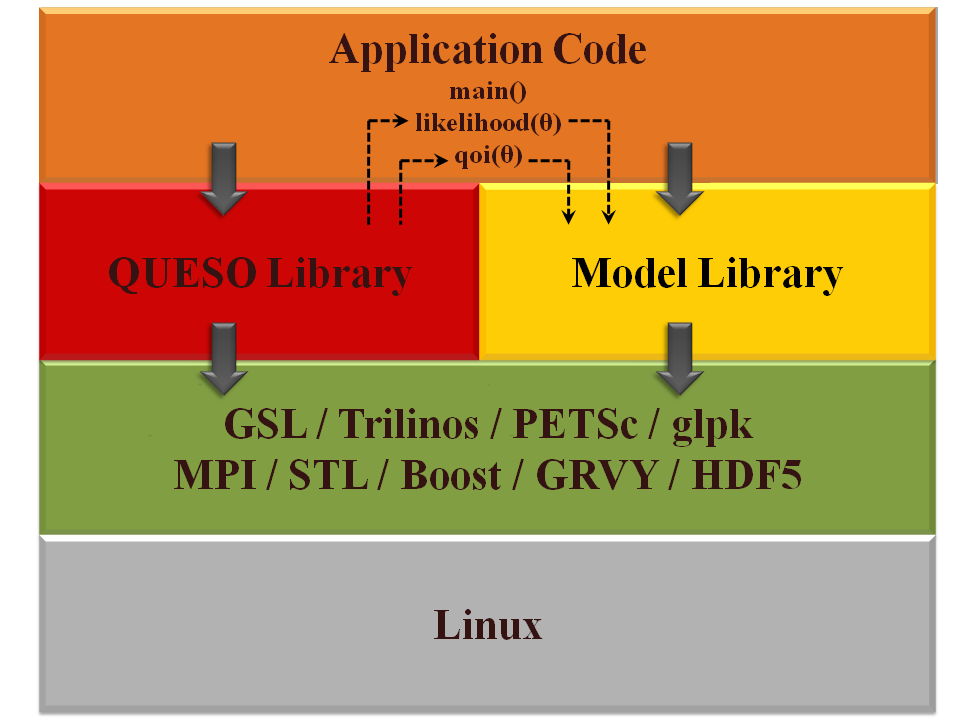
\includegraphics[scale=0.4,clip=true]{figs/quesoSwStack_09_2010.png}
}
\caption{
An application software stack.
QUESO requires the input
%supply
of a likelihood routine $\pi_{\text{like}}:\mathbb{R}^n\rightarrow\mathbb{R}_+$ for IPs and 
of a QoI routine $\mathbf{q}:\mathbb{R}^n\rightarrow\mathbb{R}^m$ for FPs.
These application level routines provide the bridge between
% among
the statistical algorithms in QUESO,
physics 
%model
knowledge in the model library, and relevant 
experimental (calibration
    and validation) data.
%model specific data in the disk space.
}
\label{fig-sw-stack}
\end{figure}

% \begin{figure}[h!]
% \centerline{
% 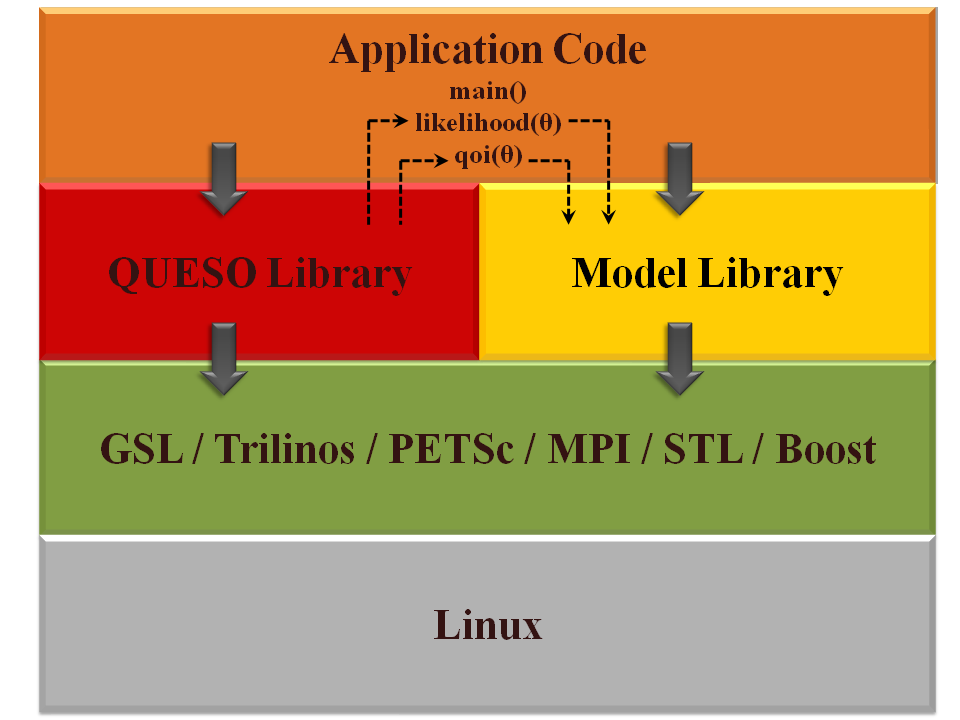
\includegraphics[scale=0.50,clip=true]{figs/queso_paper1_03}
% }
% \caption{
% Overview of the software stack of a typical application that uses QUESO.
% The symbol $\boldsymbol{\theta}$ represents a vector of $n\geqslant 1$ parameters.
% Algorithms in the QUESO library require the supply
% of a likelihood routine $\pi_{\text{like}}:\mathbb{R}^n\rightarrow\mathbb{R}_+$ for statistical inverse problems and 
% of a qoi routine $\mathbf{q}:\mathbb{R}^n\rightarrow\mathbb{R}^m$ for statistical forward problems. These routines
% exist at the application level and provide the necessary bridge between the statistical algorithms in QUESO,
% model knowledge in the model library and scenario and experimental data in the disk space.
% Concepts are further detailed in Chapter \ref{ch-introduction}.
% }
% \label{fig-sw-stack}
% \end{figure}
%
Even though QUESO deals directly with $\boldsymbol{\theta}$ and $\mathbf{q}$ only,
it is usually the case the one of the other three vectors ($\mathbf{u}$, $\mathbf{y}$ and $\mathbf{d}$) will have the biggest number of components and will therefore
dictate the size of the minimum parallel environment to be used in a problem.
%
So, for example, even though one processor might be sufficient for handling $\boldsymbol{\theta}$, $\mathbf{y}$, $\mathbf{d}$ and $\mathbf{q}$,
eight processors at least might be necessary to solve for $\mathbf{u}$.
QUESO currently only requires that the amounts $n$ and $m$ can be handled by the memory available to one processor,
which allows the analysis of problems with thousands of parameters and QoIs, a large amount even for state of the art UQ algorithms.

QUESO currently supports three modes of parallel execution:
an application user may simultaneously run:
\begin{description}
\item[(a)] multiple instances of a problem where the physical model requires a single processor, or
\item[(b)] multiple instances of a problem where the physical model requires multiple processors, or
\item[(c)] independent sets of types (a) and (b).
\end{description}

For example, suppose an user wants to use the Metropolis-Hastings (MH) algorithm to solve a statistical IP, and that 1,024 processors are available.
If the physical model is simple enough to be handled efficiently by a single processor, then the user can run 1,024 chains simultaneously, as in case (a).
If the model is more complex and requires, say, 16 processors, then the user can run 64 chains simultaneously, as in case (b), with 16 processors per chain.
QUESO treats this situation by using only 1 of the 16 processors to handle the chain.
When a likelihood evaluation is required, all 16 processors call the likelihood routine simultaneously.
Once the likelihood returns its value, QUESO puts  15 processors into idle state until the routine is called again or the chain completes.
Case (c) is useful, for instance, in the case of a computational procedure involving two models,
where a group of processors can be split into two groups, each handling one model.
Once the two-model analysis end, the combined model can use the full set of processors.\footnote{The parallel capabilities of QUESO have been exercised on the Ranger system of the TACC \cite{tacc} with up to 16k processors \cite{ChOlPr10}.}


